%%%%%%%%%%%%%%%%%%%%%%%%%%% asme2ej.tex %%%%%%%%%%%%%%%%%%%%%%%%%%%%%%%
% Template for producing ASME-format journal articles using LaTeX    %
% Written by   Harry H. Cheng, Professor and Director                %
%              Integration Engineering Laboratory                    %
%              Department of Mechanical and Aerospace Engineering    %
%              University of California                              %
%              Davis, CA 95616                                       %
%              Tel: (530) 752-5020 (office)                          %
%                   (530) 752-1028 (lab)                             %
%              Fax: (530) 752-4158                                   %
%              Email: hhcheng@ucdavis.edu                            %
%              WWW:   http://iel.ucdavis.edu/people/cheng.html       %
%              May 7, 1994                                           %
% Modified: February 16, 2001 by Harry H. Cheng                      %
% Modified: January  01, 2003 by Geoffrey R. Shiflett                %
% Modified: July 19, 2009 as a template in a single column for       %
%           ASME Journals by Harry H. Cheng                          %
% Use at your own risk, send complaints to /dev/null                 %
%%%%%%%%%%%%%%%%%%%%%%%%%%%%%%%%%%%%%%%%%%%%%%%%%%%%%%%%%%%%%%%%%%%%%%

%%% use 10pt options with the asme2ej format
%\documentclass[10pt]{asme2ej}
\documentclass[12pt,cleanfoot,twocolumn]{asme2ej}

\usepackage{graphicx} %% for loading jpg figures
\usepackage{epsfig}
\usepackage{fancyhdr}
\usepackage{setspace}
\usepackage{helvet}
\usepackage{fontspec}
\usepackage{float}
\usepackage{xeCJK}
\usepackage[hyphens]{url}
%\usepackage{hyphens}
\renewcommand{\familydefault}{\sfdefault}
\usepackage{hyperref}
\hypersetup{
    colorlinks=true,
    linkcolor=blue,
    urlcolor=blue,
    pdftitle={Overleaf Example},
    pdfpagemode=FullScreen,
}
\pagestyle{fancy}
\rhead{}
\renewcommand{\headrulewidth}{0pt}
\topmargin 80 pt
\headheight 14 pt
\headsep 30 pt
\setmainfont{Times New Roman}
\setCJKmainfont{Microsoft JhengHei UI}
\XeTeXlinebreaklocale "zh"
\XeTeXlinebreakskip = 0pt plus 1pt
\graphicspath{ {./figure/} }
%\RequirePackage[hyphens]

%% The class has several options
%  onecolumn/twocolumn - format for one or two columns per page
%  10pt/11pt/12pt - use 10, 11, or 12 point font
%  oneside/twoside - format for oneside/twosided printing
%  final/draft - format for final/draft copy
%  cleanfoot - take out copyright info in footer leave page number
%  cleanhead - take out the conference banner on the title page
%  titlepage/notitlepage - put in titlepage or leave out titlepage
%  
%% The default is oneside, onecolumn, 10pt, final


\title{文字探勘初論 期末專案\\
        政治新聞分類系統}

\author{蕭瑀
\affiliation{
        系級: 資管四\\
        學號: B08705059
}}

\author{張力升
\affiliation{
    系級: 資管三\\
    學號: B09705007
}}

\author{李彥澂
\affiliation{
    系級: 資管三\\
    學號: B09705012
}}

\author{蔣詠心
\affiliation{
    系級: 資管三\\
    學號: B09705020
}}

\author{許圃菘
\affiliation{
        系級: 資管三\\
        學號: B09705027
}}

\author{陳亮妤
\affiliation{
        系級: 資管三\\
        學號: B09705033
}}
    
\begin{document}

\maketitle

\section{Purpose of the project}
有鑒於我們這組的組員大多都是今年 11 月底九合一大選的首投族,剛獲得投票權的我們躍躍欲試,希望可以投下手中神聖的一票,但我們真的有好好把握我們手中的選票嗎?在選舉前一兩週,我們發現我們自己跟身邊的人對於政治似乎沒有太大的興趣。已經都快要選舉了,連總共有幾位市長候選人都不清楚,因此希望可以找出一種模式讓大家更接近政治、知道現在選情的熱度,以及更了解候選人,讓我們手中這一票不是隨便地投給任何一位看得順眼的人,而是真正了解過候選人看法、政見等做出的決定。

而新聞是最容易傳播資訊的媒體,也是傳遞資訊的主流管道。近幾年因網路科技發達,網路新聞崛起,數量非常地多,但每次在網站上總是只看得到一些存得亂七八糟,或是把相關的新聞放得很散的情況。

因為文字探勘初論期末報告主要著墨在文章的分類,還有可以利用爬蟲取得的特性,所以這次的期末專案選定以網路上的文字新聞為主要資料來源,以其內容作為我們要判斷的文章。透過幫大家整理政治主題的新聞,把有相關的文本收集起來,用分類就可以讓大家很容易地使用我們網站,找到自己有興趣的關鍵字的相關新聞。

\section{Solution}
為了不讓專案規模太大,這次專案先專注於「新竹市市長選舉」。

\subsection{資料集}
\subsubsection{資料來源與範圍}
資料來源為「自由時報」、「聯合報」的網站,範圍是報導發布時間介於 2022/6/1 到 2022/11/25、內容和新竹市長選舉相關的新聞。總共蒐集了 2787 篇新聞。

\subsubsection{Label}
我們根據報導的標題及內文所指涉的主題,在其中 1000 篇新聞上標了 Label。因為新聞內容可能同時提及多個主題,我們決定讓每篇新聞可以有複數個主題,或者沒有主題。Lable 總共有三種:
\begin{itemize}
        \item 選情:單純分析選情之新聞。
        \item 事件:跟特定事件相關的新聞,事件例子為「林智堅論文抄襲爭議」、「高虹安助理費爭議」等。
        \item 政策:跟候選人提出的政見相關的新聞。
\end{itemize}
選擇這三個主題做為 label 並不是空穴來風:我們一開始的構想是專注於跟「政見」相關的新聞,把關於不同類型政見的新聞分類,好讓民眾查詢。例如民眾可以查「交通」,那麼就會出現關於「新竹輕軌」、「跨縣市大橋」等相關新聞。但後來遇到兩個問題,首先是台灣媒體對於候選人的政見並沒有太多著墨,蒐集資料有困難。後來我們改變方向變成分析「所有」新竹市長選舉的相關新聞,並分出大約 13 個類別,但後來發現政治新聞內容比較鬆散,13 個類別中有許多類別文章很少,訓練 SVM 的效果很差。最後才決定找三個最大的主題當作 Label。

\subsection{Tokenization}
因為文本內容為中文,因此我們選擇使用 Jieba 進行 tokenization。但 Jieba 主要是針對簡體中文,且我們使用的情境中會出現大量的政治詞彙,因此我們自己手動加入了 472 個詞彙幫助 tokenization。這些詞彙中包含了本次九合一選舉中常常出現的詞彙,例如「九合一」、「樁腳」、「公積金」、「三角督」等,也包含了跟台灣政治人物、政黨:「林耕仁」、「高虹安」、「沈慧虹」、「民進黨」、「國民黨」、「民眾黨」等等。
增加這些詞彙後,Jieba 切出來的 token 大多都是正確的。

\subsection{Vectorize}
\subsubsection{TF-IDF vector}
我們使用 sklearn 提供的 TfidfVectorizer 將 2787 篇文章切出來的 token 轉換成 TF-IDF vector。最後的字典維度是 56175 維。

\subsubsection{SVD vector}
接下來我們使用 sklearn 提供的 TruncatedSVD 將 TF-IDF vector 轉成 SVD vector,將維度從 56175 維降成 100 維。

\subsection*{Classification}
因為每篇文章可以有複數個主題,或是沒有主題,因此我們對「選情」、「事件」、「政策」這三個分別二元分類。
Model 選擇使用 SVM。我們使用 1000 篇有標 label 的文章中的 900 篇進行 model selection(選 kernel)以及 tuning,最後選出來的 model 結果如下:
\\
\begin{center}
        \begin{tabular}{c|c|c|c}
                Label & Kernel & $C$  & $\gamma$ \\
                \hline
                選情  & RBF    & $10$ & $0.1$    \\
                事件  & RBF    & $1$  & $1$      \\
                政策  & Linear & $1$  &          \\
        \end{tabular}
\end{center}

\section{System outcomes}
\subsection{Precision \& Recall}
我們使用剩下的 100 篇文章做 testing,結果如下:
\begin{center}
        \begin{tabular}{c|c|c}
                Label & Precision & recall \\
                \hline
                選情  & $0.77$    & $0.80$ \\
                事件  & $0.95$    & $0.82$ \\
                政策  & $0.88$    & $0.62$ \\
        \end{tabular}
\end{center}
三個 Label 中以「事件」的效果為最佳,precision 甚至達到 0.95。「選情」跟「政策」則是 precision 跟 recall 都較低。

\subsection{Curve}
我們也將結果畫成 Precision recall curve:
\begin{figure*}
        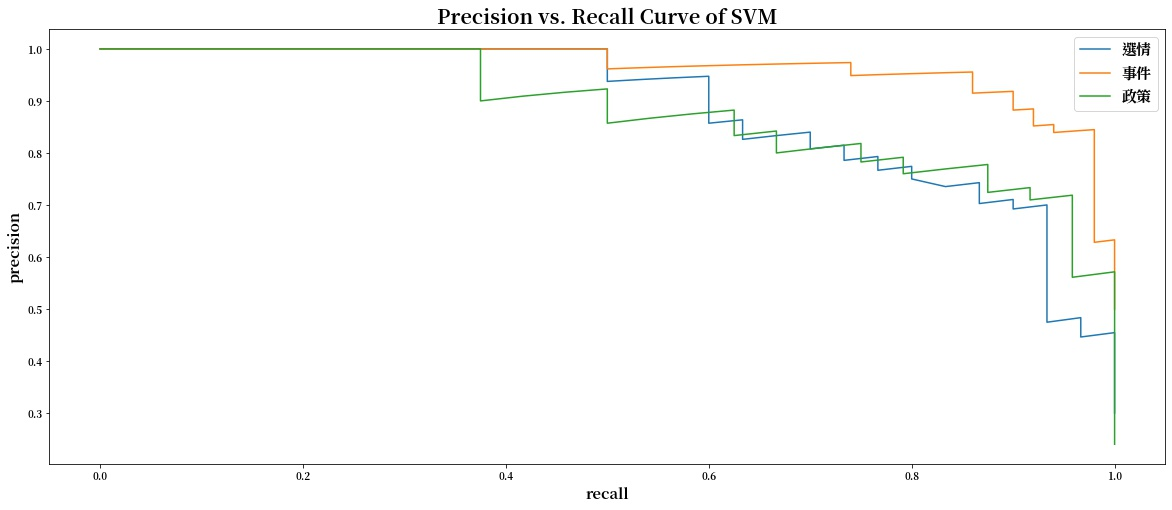
\includegraphics[width=\textwidth]{pr_curve}
\end{figure*}

從圖中可以看到「事件」類別 model 較有把握的真的都判對,且效果比另外兩個 Label 明顯好蠻多的。

\section{Conclusions}
分類的效果以「事件」類別最佳,我們推測主要有兩個原因:
\begin{enumerate}
        \item 「事件」類別的新聞較多:在 $900$ 筆訓練資料中,有 $448$ 筆屬於「事件」類別。反觀「選情」及「政策」,分別只有 $365$ 篇及 $199$ 篇。
        \item 「事件」類別的關鍵字較為集中:事件類別大多都會針對同一候選人、同一爭議。在標資料的過程中,「林智堅」、「高虹安」、「論文」、「抄襲」、「公積金」、「助理費」、「資策會」等等關鍵字也時常反覆出現,因此猜測在向量空間中,這些關鍵字雖然被降維了,但還是有很重的份量,導致「事件」類別較容易判讀。而「選情」、「政策」類別內容則可能較為分散,尤其是政策,很多文章都只有簡單提到一些重點政見的 slogan,很少文章有花大篇幅說明政見,因此在向量空間中,「政策」類別可能較為零散
\end{enumerate}


\section{web page}
最後有將網頁實作出來,並將剩下的 1787 篇沒有標 label 的文章丟到訓練好的 model 中分類。

\subsection{初始頁面}
進入初始頁面後,可以選擇想要查看的縣市。目前只有新竹市有資料
\begin{figure}[H]
        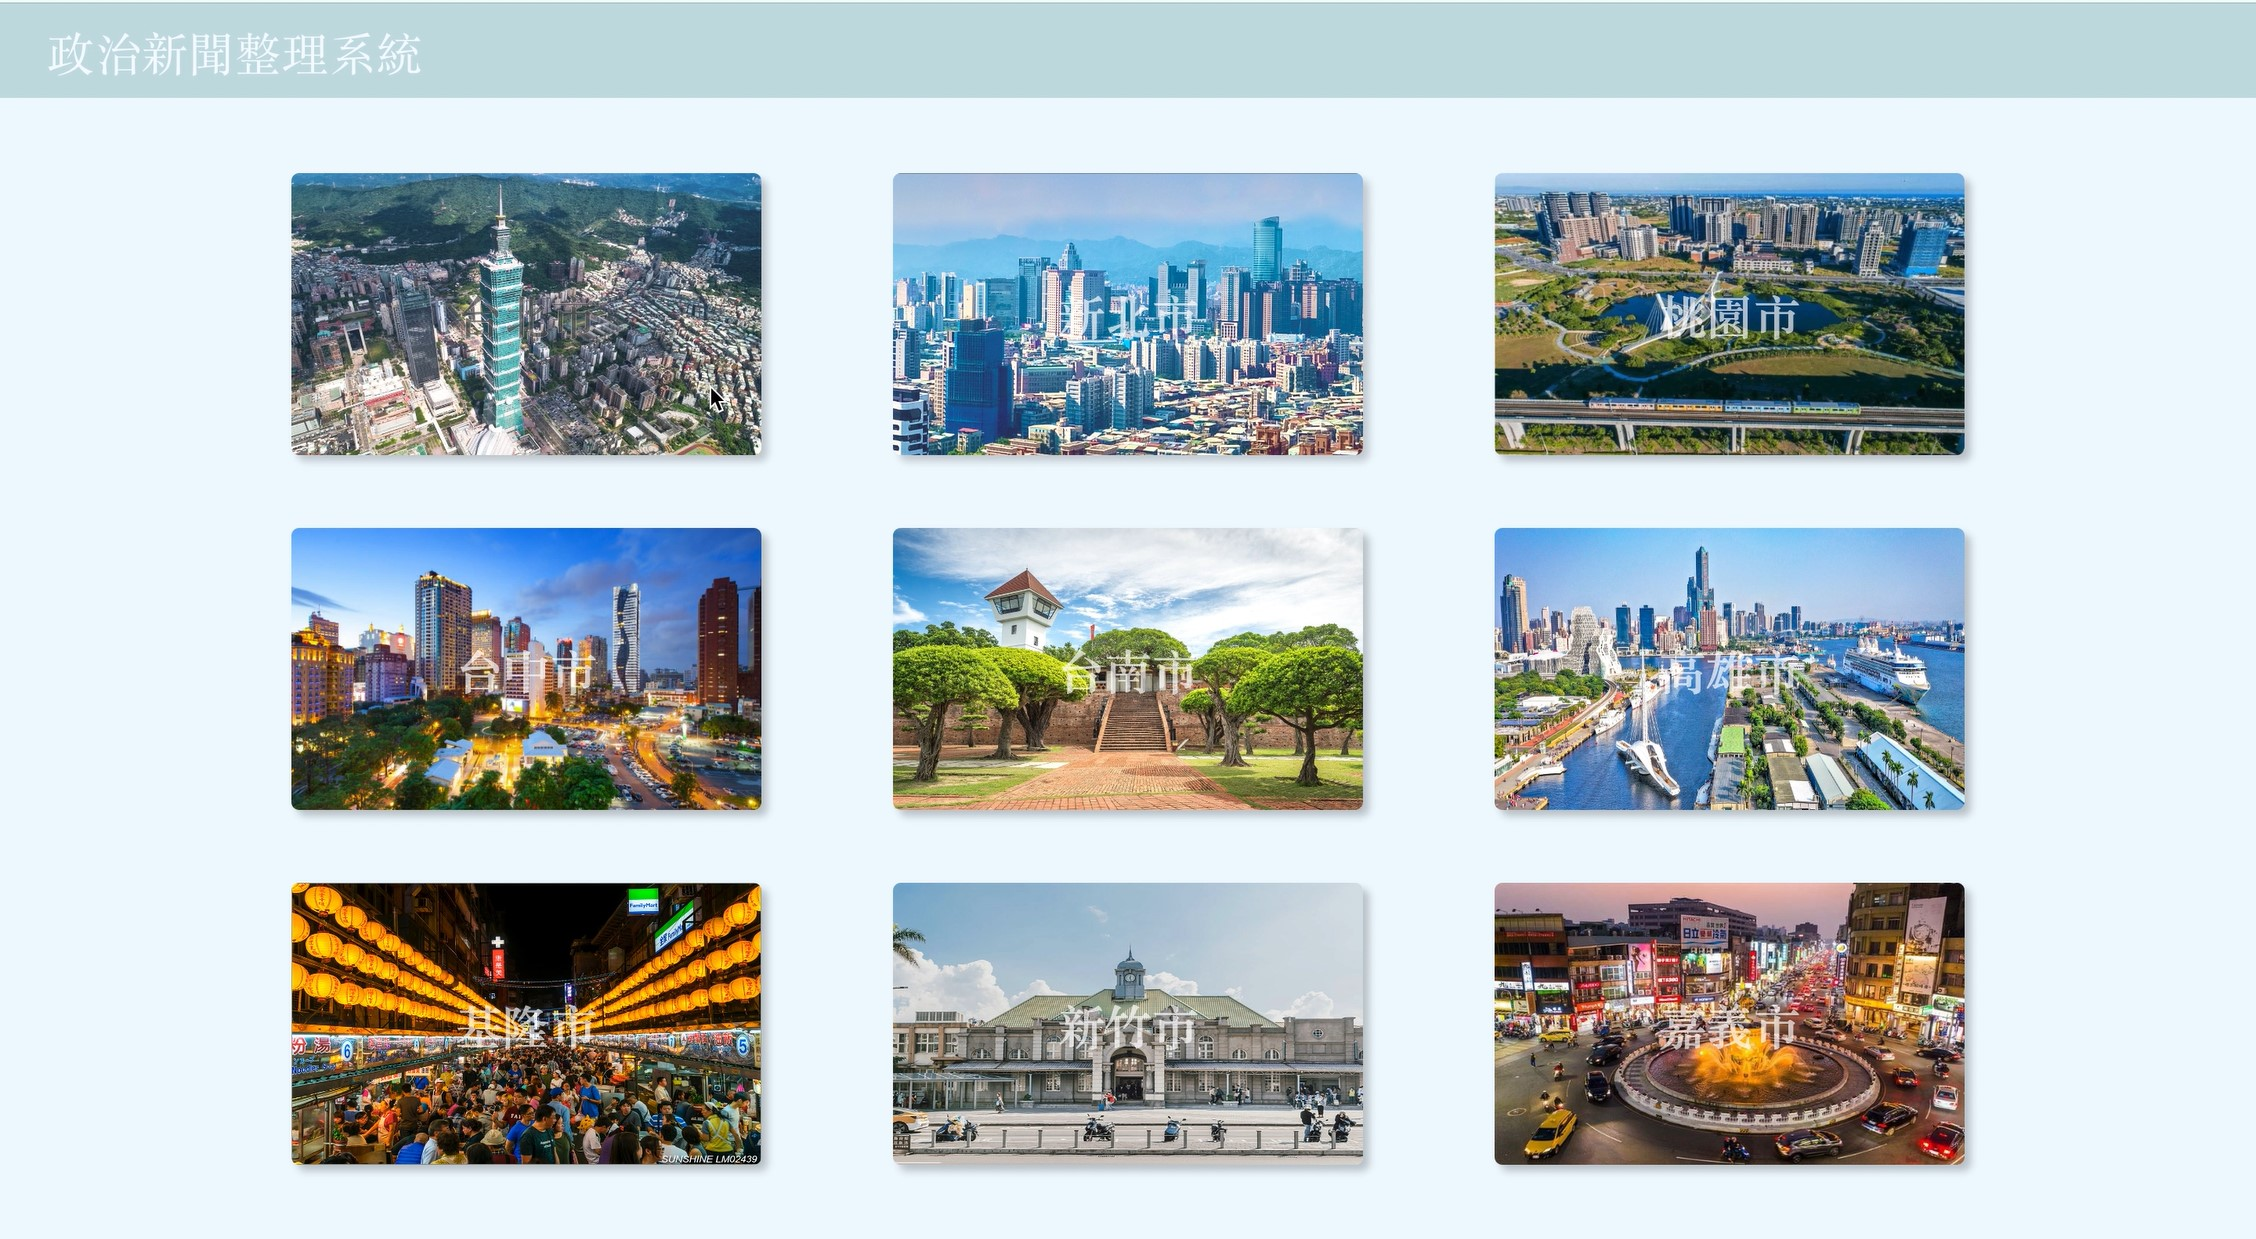
\includegraphics[scale=0.2]{start}
        \caption{初始頁面}
\end{figure}
\subsection{某縣市類別頁面}
點擊該縣市後,即可進入該縣市的類別頁面。在這個頁面中會秀出「選情」、「事件」、「政策」類別中的其中一些新聞

\begin{figure}[H]
        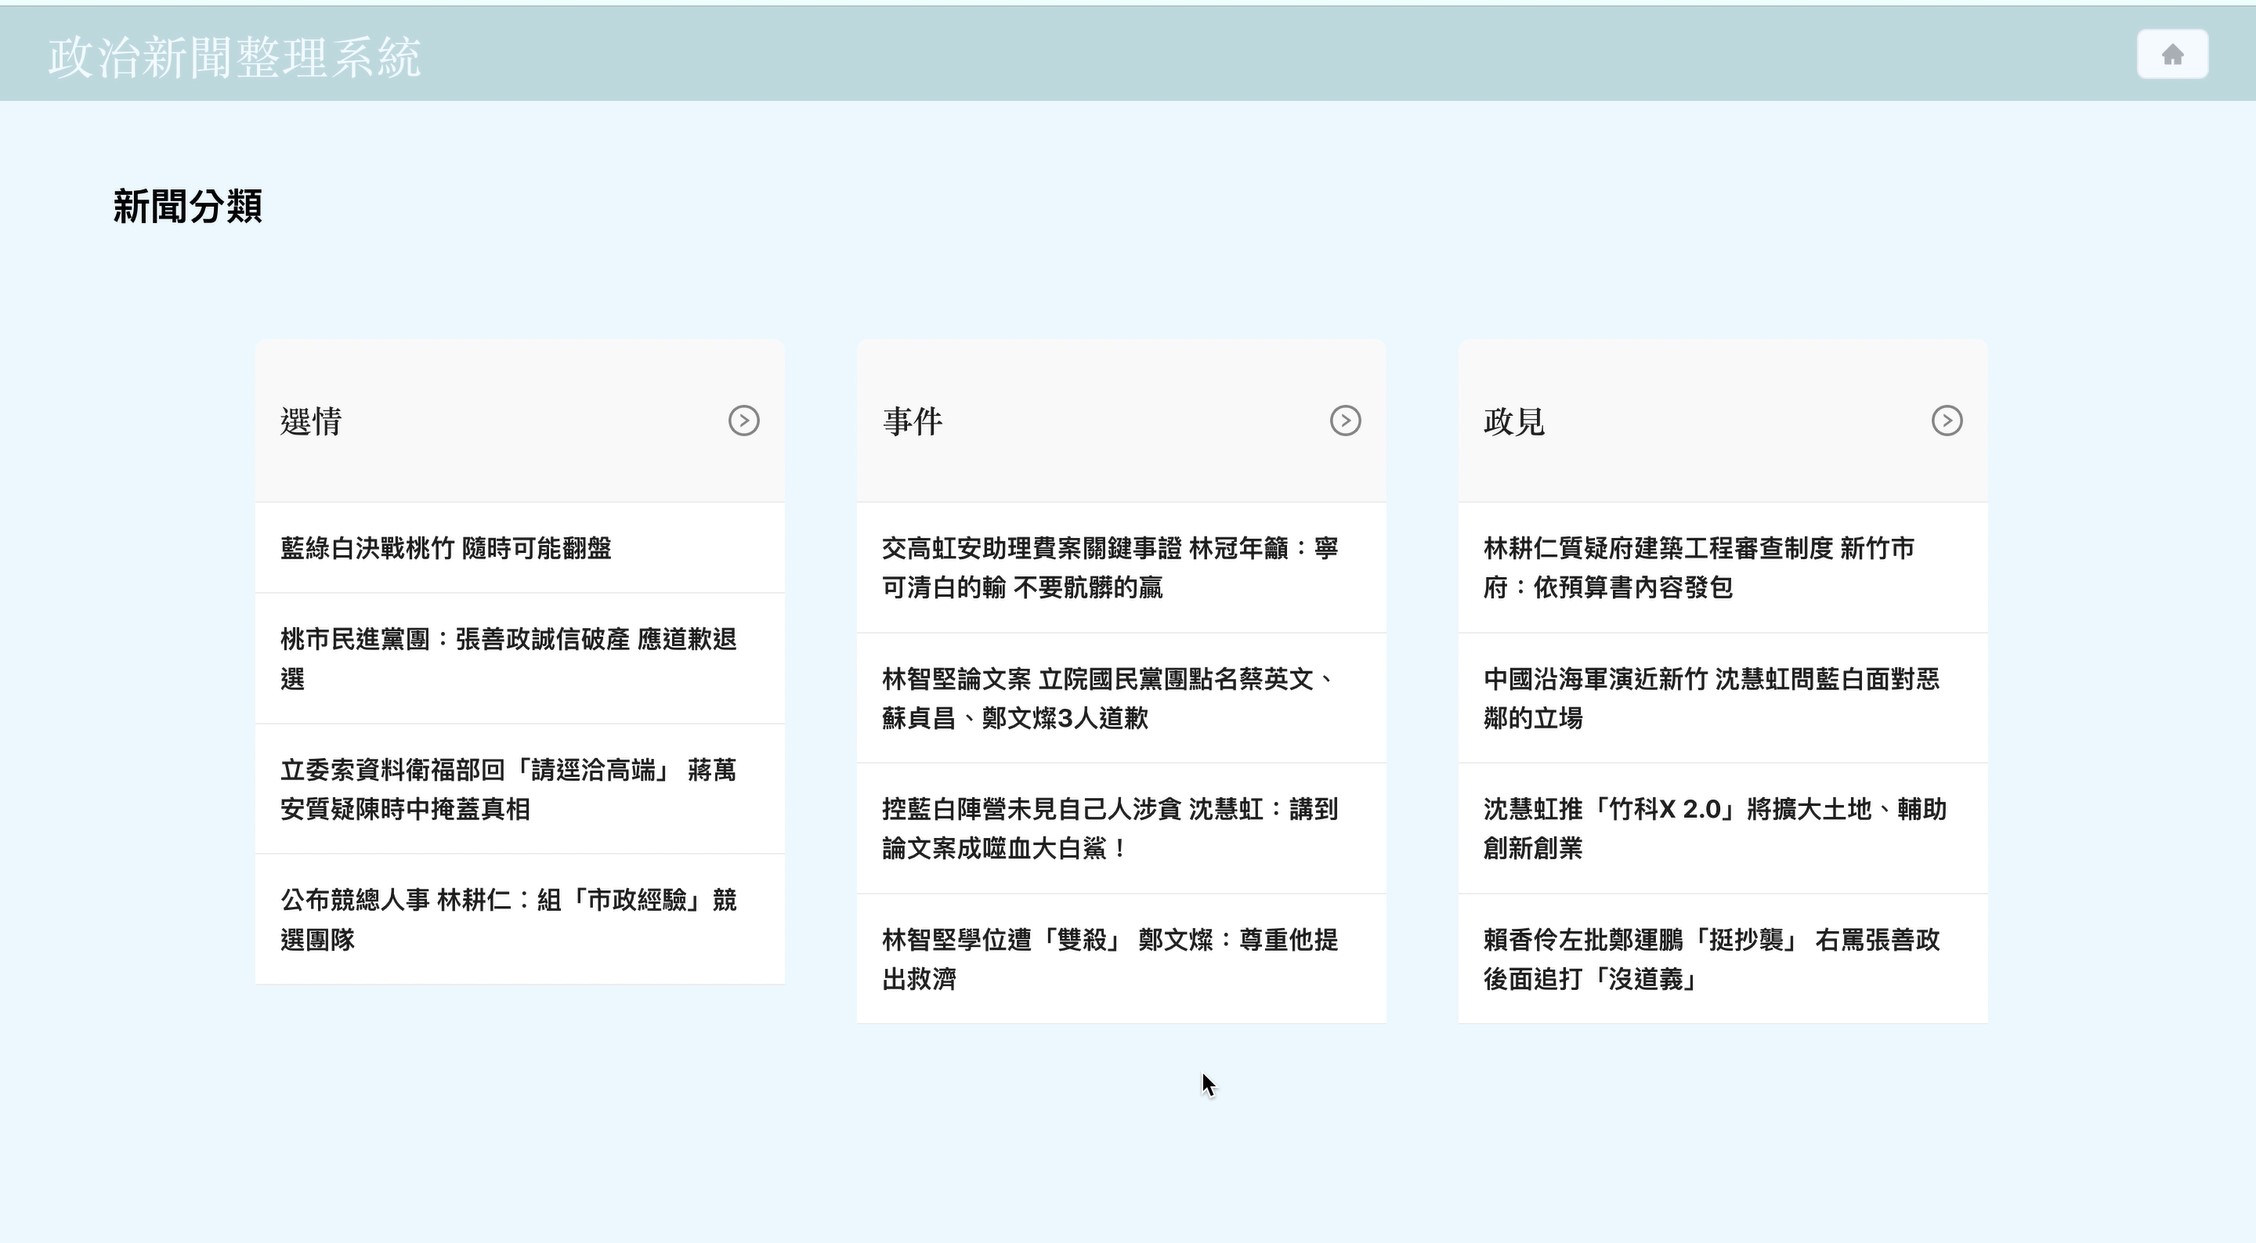
\includegraphics[scale=0.2]{outline}
        \caption{新竹市類別頁面}
\end{figure}

\subsection{類別新聞}
選擇某個類別,可以進入該類別的頁面。裡面會顯示所有屬於這個類別的新聞。
下圖是進入了「事件」的類別,可以看到圖中有許多關於林智堅論文爭議的新聞。

\begin{figure}[H]
        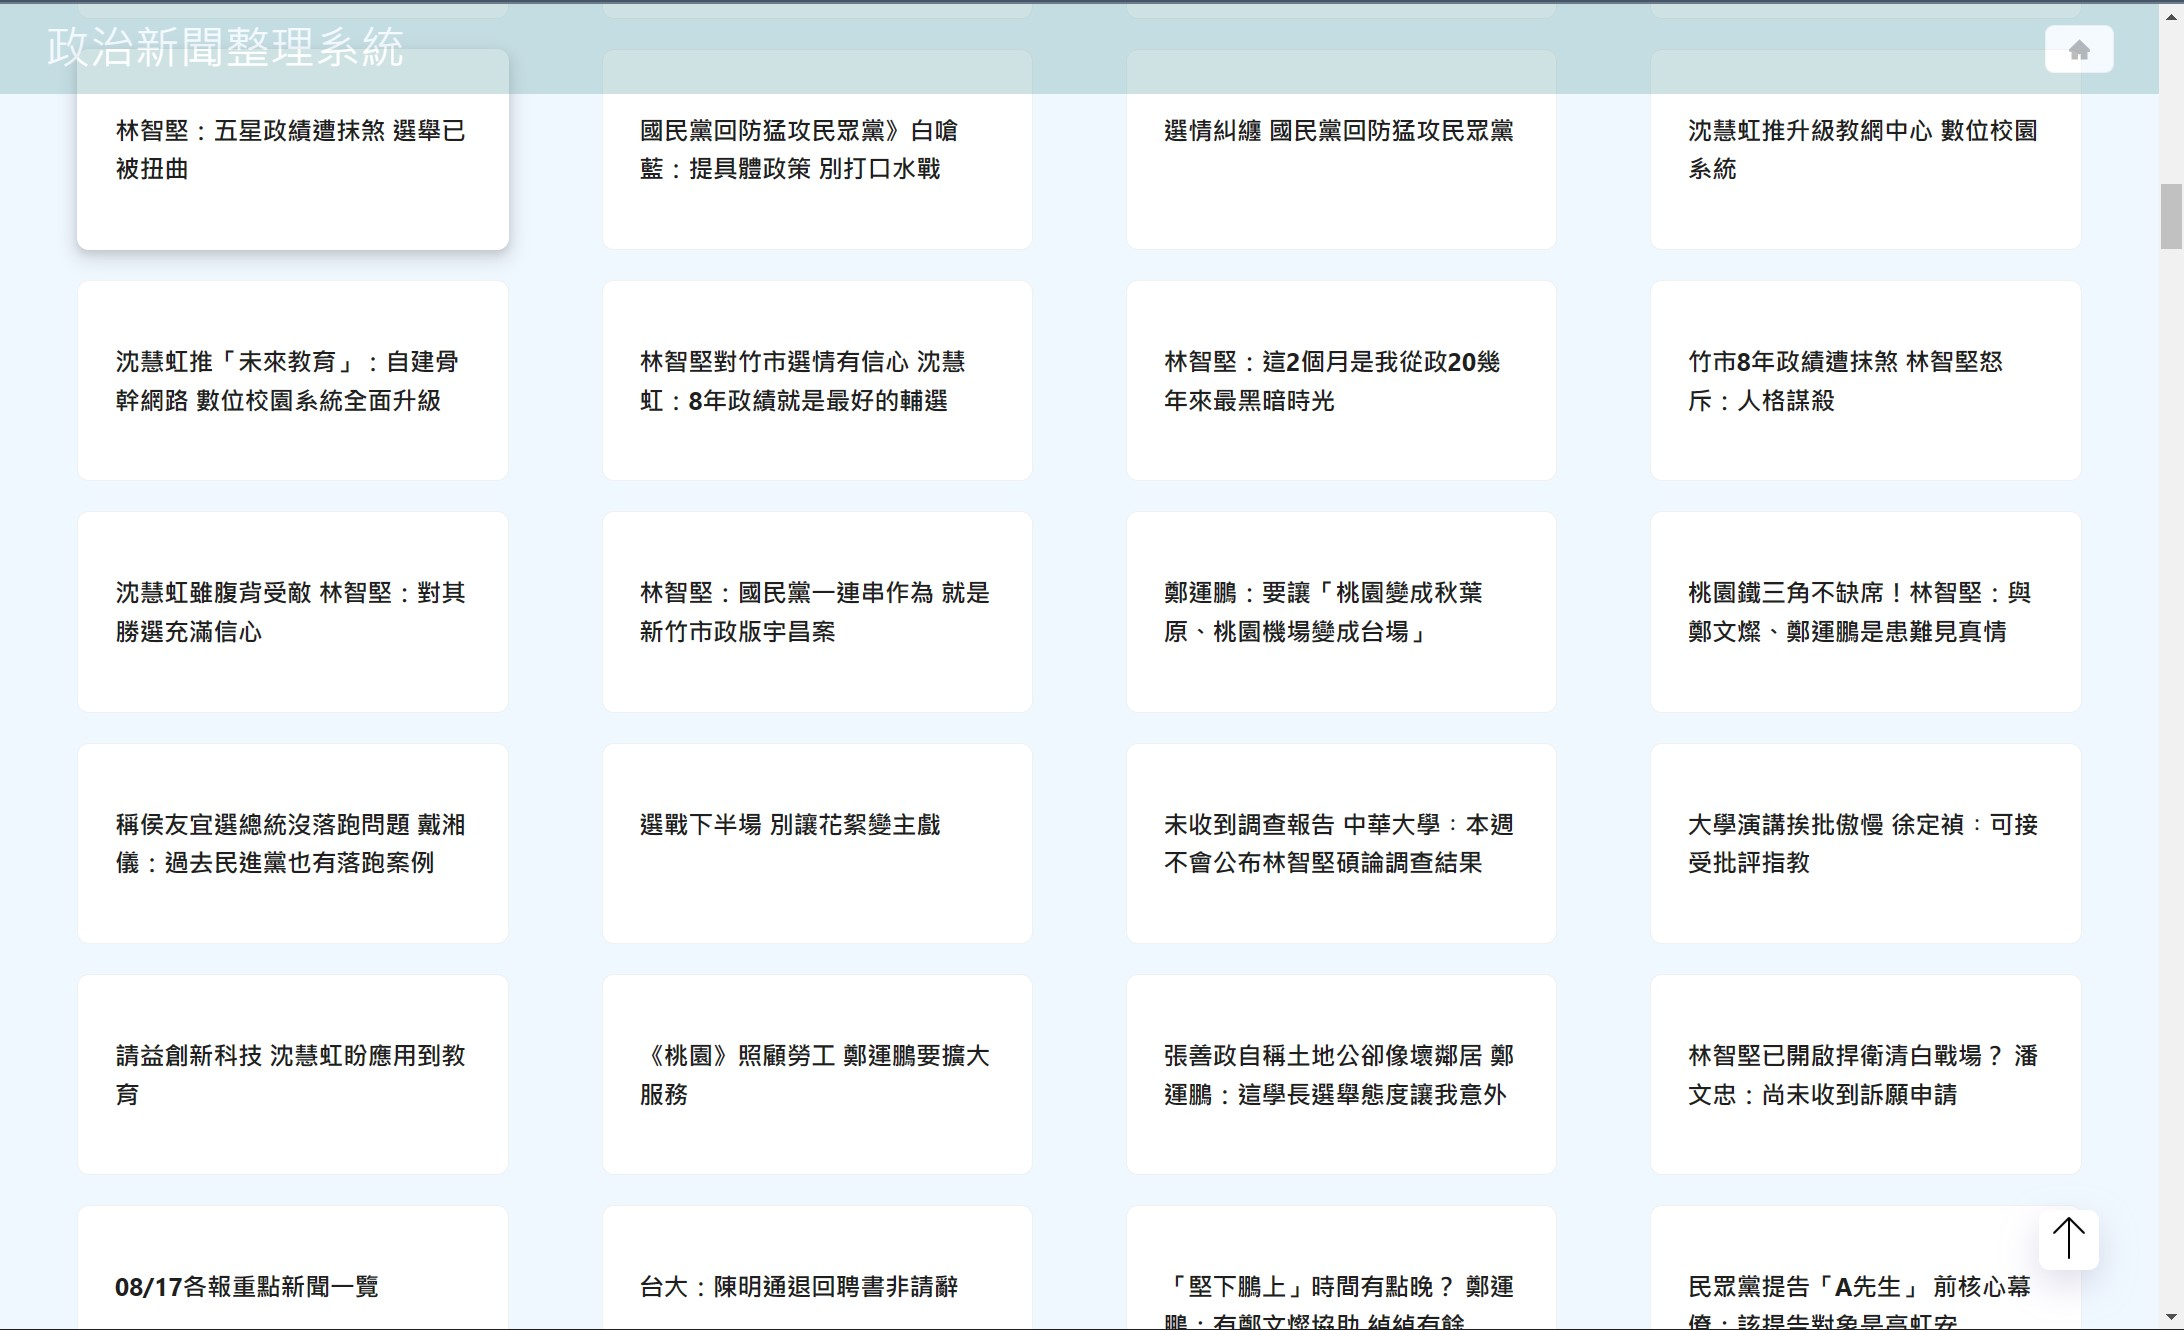
\includegraphics[scale=0.2]{event}
        \caption{「事件」類別新聞}
\end{figure}

\subsection{瀏覽新聞}
選擇某一則新聞即可瀏覽全文,也會附上該篇新聞的連結。

\begin{figure}[H]
        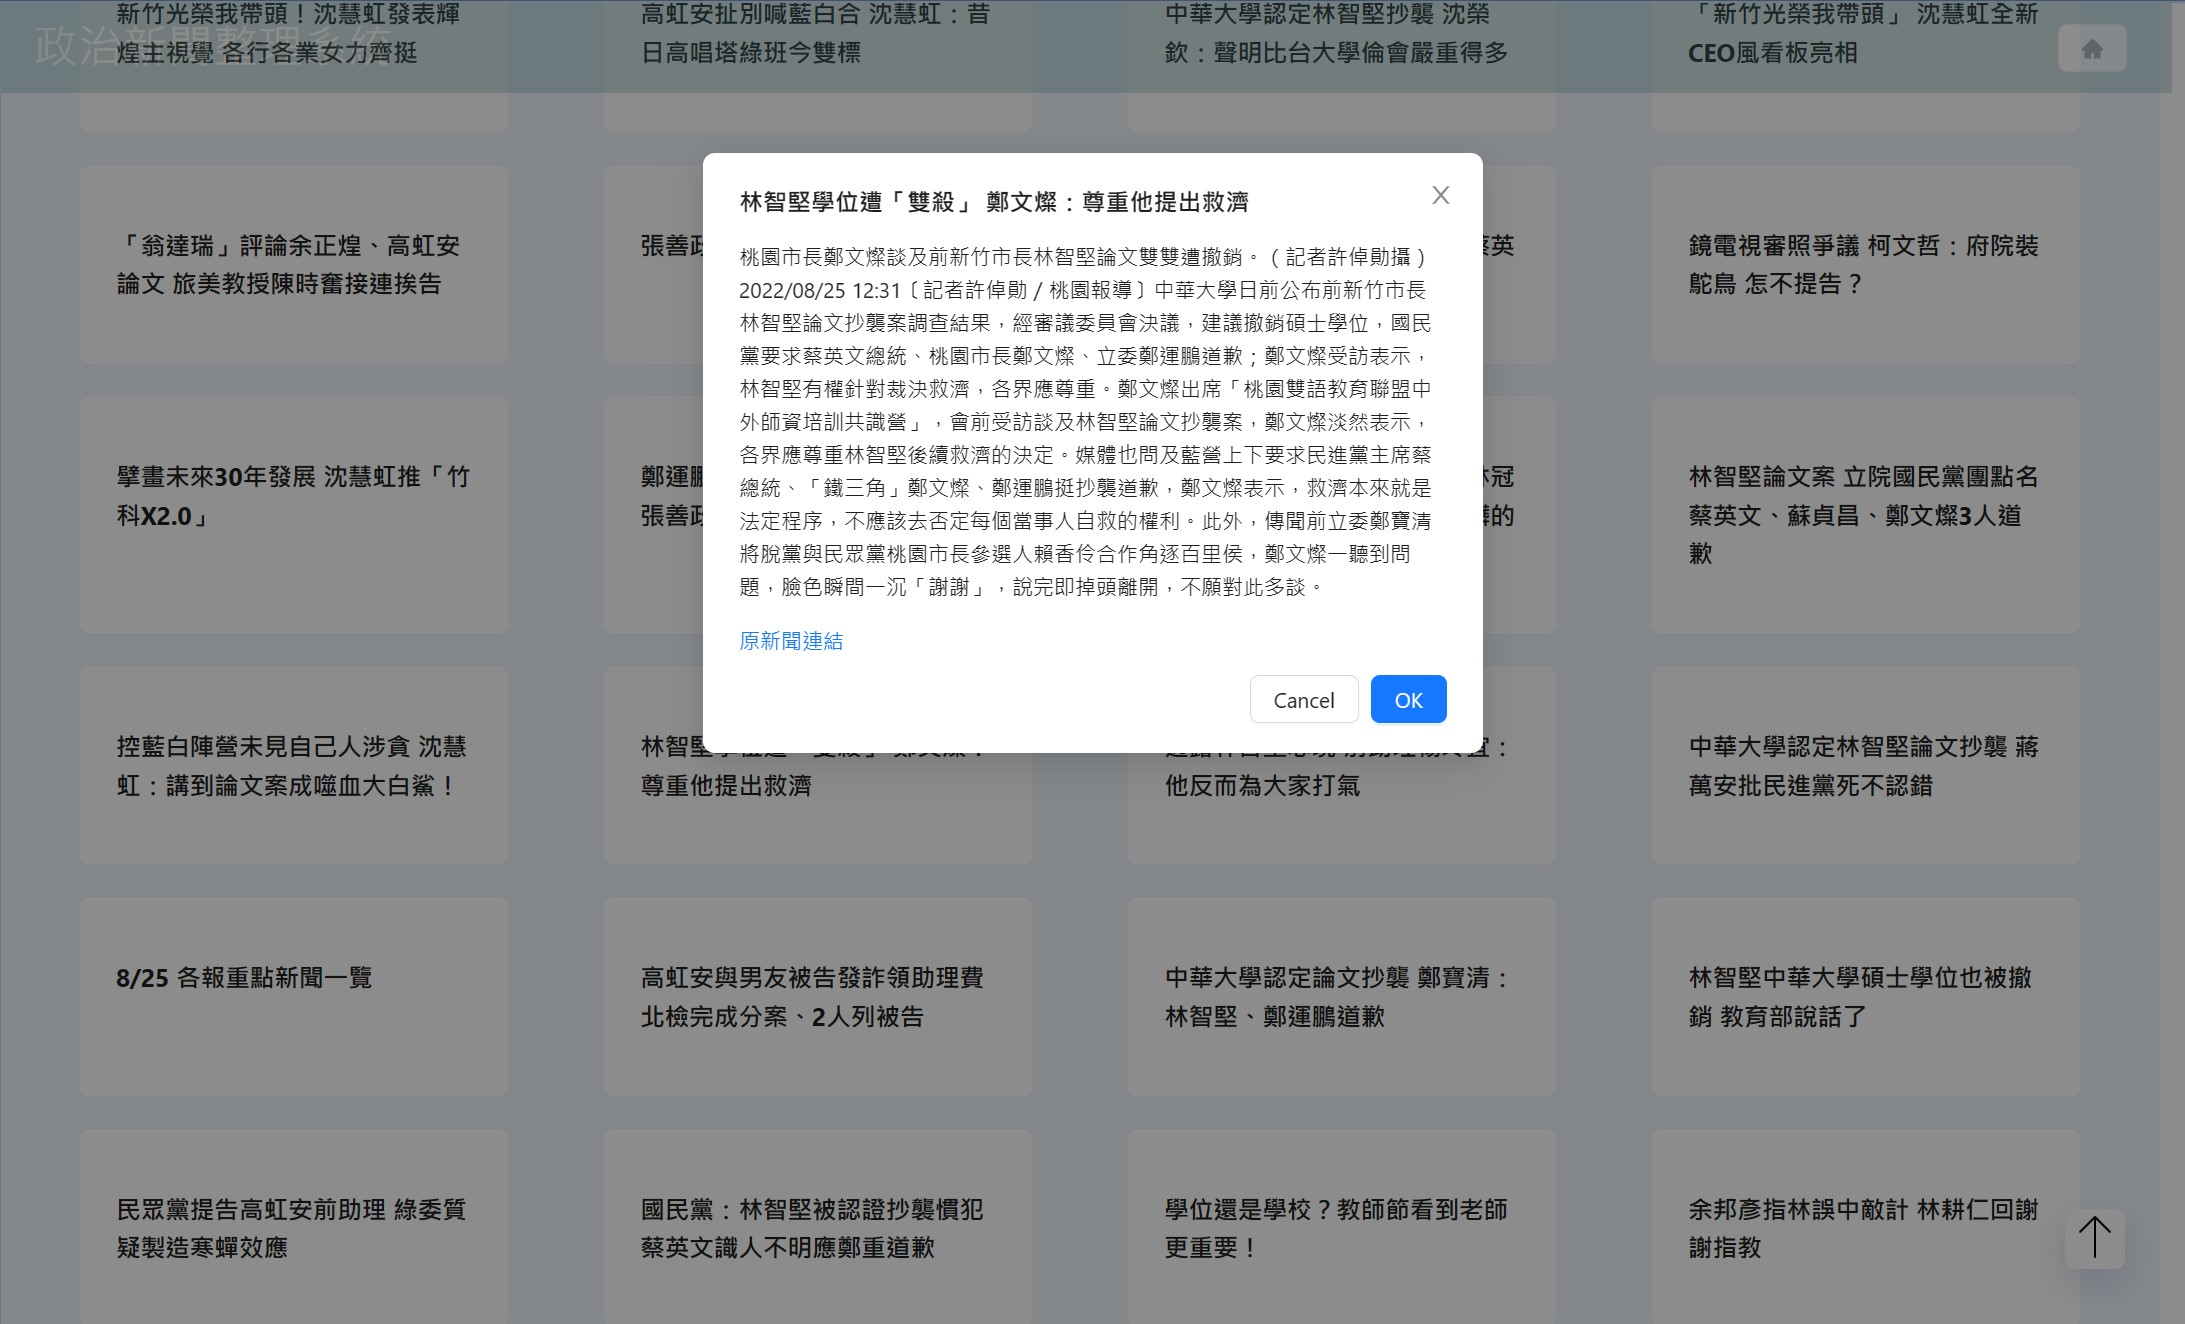
\includegraphics[scale=0.2]{news}
        \caption{瀏覽新聞}
\end{figure}

\section{References}
Seung-Shik Kang, ``Keyword-based Document Clustering" \\
(原本打算用 clustering 將不同政策分群,但後來改變方向就沒有使用了)
\end{document}